\chapter{Complex event processing}
\label{chap:cep}

Chapter
\section{Formal Intro of the Event Automatons}
	In our hierarchical runtime verification project, the top (Highest?) level of modelling is done in an event pattern language.
	This pattern language will be compiled to Calender Event Automatons.
	\subsection{Current Formalisms}
		% valami bevezeto a dologhoz?
		\subsubsection{Event Automaton}
			An Event Automaton is a non-deterministic finite-state automaton whose alphabet consists
			of parametric events and whose transitions may be labelled with guards and assignments
		\subsubsection{Calendar Event Automaton}
			% stuff about the calendar
			In discrete event simulation, a calendar (also called event list) is a data structure that
			stores future events and the times at which these events are scheduled to occur
			% stuff about the calender automaton
			
	\subsection{Our Formalism}

\section{Examples of Event Processing}

	\subsection{File System}
	\begin{figure}[h]
	\centering
	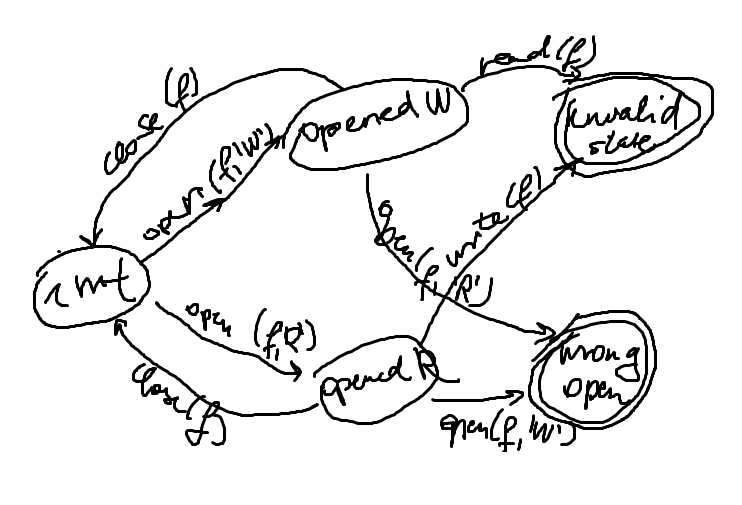
\includegraphics[width=0.5\linewidth]{include/figures/chapter_5/fileautomaton}
	\caption{Automaton of the file examplee}
	\label{fig:cep:fileautomaton}
	\end{figure}

	Consider the following example : We have a file system, with the following parameterized events : open(mode,file),close(file),read(file),write(file)
	\subsection{Mars Rover Tasking}

\section{Implementation}
	\subsection{Metamodel}
	%image
	\subsection{Executor}
